\documentclass[11pt]{article}
\usepackage{graphicx}
\usepackage[left=0.5in,right=0.5in,top=1in,bottom=1in]{geometry}
\usepackage{amsmath}
\begin{document}

\title{Project Report For Cs296}

\author{
	Vishal Rajiv Agarwal\\
	120011009\\
	\texttt{120110009@iitb.ac.in}
	\and
	Jagadeesh Nelaturu\\
	120050055\\
	\texttt{nssjagadeesh@iitb.ac.in}
	\and
	Nishanth Rumandla\\
	120050064\\
	\texttt{120050064@iitb.ac.in}}

\date{\today}

\maketitle

\section{Introduction}
	In this report we present our Box 2D simulation of a JCB. We talk about our original design, our final design, the differences among them, some interesting feautres of our design etc. We further do a statistical analysis of our simulation using Gnuplot. We also analyze the running time of our simulation using profilers like gprof.  
\section{Our Original Design}
	Our original design was inspired from an animation of a JCB which we found online. We then went ahead and made our own 2D picture of it. The picture below is our original design. Our orignal design had eight degrees of freedom along with a few objects which we would pick using our JCB. 
	\begin{center}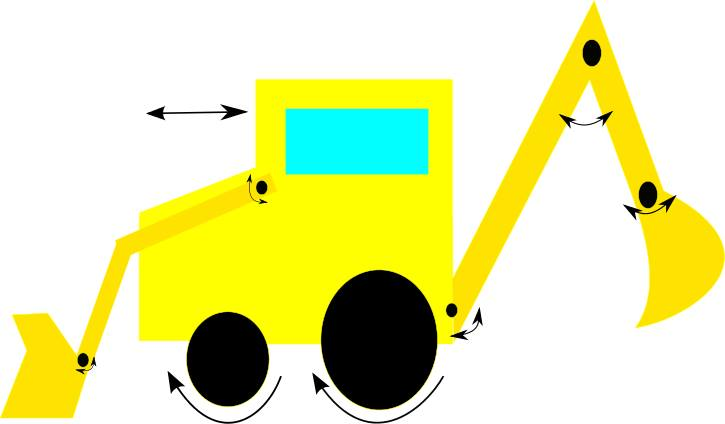
\includegraphics[height=6cm]{BullDozerDesign.jpg}\end{center}
\section{Our Final Design}
	In the subsections to follow we talk about some interesting features of our simulation, differences between our orginal design and our final design, some drawbacks of our original design and some challenges we faced while making the simulation. The picture below is a screenshot of our simulation.
	\begin{center}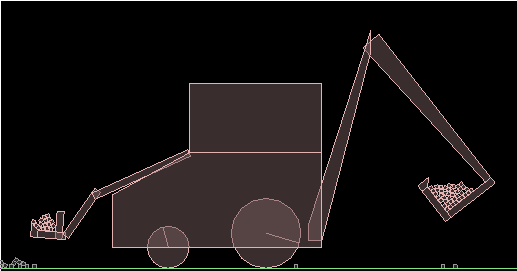
\includegraphics[height=5cm]{FinalDesign2.png}\end{center}
	\subsection{What Makes Our Design Interesting}
	One of the most interesting feature of our design is that the arms of the JCB seem to be levitating in air, implying they act as if they are not affected by the force of gravity. An actual JCB has hydraulics at its disposal to facilitate this.
 Our solution to this design flaw was to use Motors in Box 2D. A motor allows a joint to act as a rusted joint where the amount of rust can be quantized. One can move the arms of the JCB by applying a large impulse (due to the rust) at the appropriate point. One major drawback of this was that when we picked objects using our JCB this impulse was also transfered to the objects. We came about this by fine tuning some physical properties of the objects like their friction coefficient and density.\newline
	An interesting feature of our design is the design of the claws. They are a hybrid of the ForkLift claw and the JCB claw. A Spoke like thing has been welded at the end of the claw to ensure that objects do not slip off when the JCB moves. The pointed end also helps in the digging action.\newline
	\begin{center}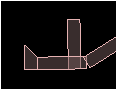
\includegraphics[height=3cm]{Left_Claw1.png}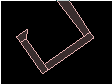
\includegraphics[height=3cm]{Right_Claw.png}\end{center}	
	Another interesting feature of our design are the callbacks which allow the user to control the JCB using the keyboard.
Various keys can be used to move different parts of the JCB. One can independently move the claws and the arms of the JCB. One can also move the entire JCB on the horizontal plane.
	\subsection{Differences Between Our Original And Final Design}
	If one observes carefully one notices that our original design had a degree of freedom at the base of the right arm unlike our final design. By adding this degree of freedom one would make the motion of the right arm very complicated. Our solution to this was to make the right sub-arm long so that it could always reach the ground to dig objects. But this limited the depth to which one could dig. Actual JCB's have this degree of freedom\cite{youtube}.
Instead we added another degree of freedom to the left sub-arm to allow free motion between the left claw and the base of the left arm.\newline
	Another difference between our original design and our final design is the shape of the right and left claws. This was because Box 2D did not allow one to construct convex polygons. An alternative to this would be to construct the shape using small bars and weld joints. This would unnecessarily complicate our design, so we choose to modify the claws to something similar to a hybrid of a JCB claw and a forklift claw\cite{wiki}.\newline
	 We added a few small boxes to our original design to represent mud, this was done so that we could test the functionality of our JCB. We neatly formed a cube of these small boxes for representational purposes.
	\begin{center}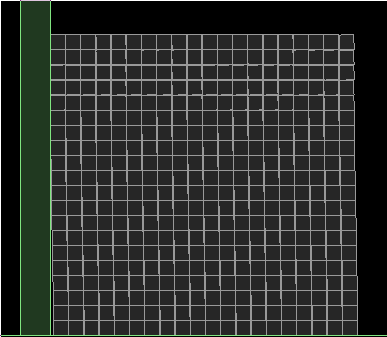
\includegraphics[height=3.5cm]{Boxes.png}\end{center}
\section{Analyzing Our Simulation Using Gnuplot}
	In the subsections to follow we analyze the running time of our simulation using five different types of graphs. We also try to explain the reasons for some interesting things we observed during the analysis of the graphs. 
	\subsection{Analyzing Loop Time And Average Step Time }
	 From the below graph it is quite clear that the total loop time increases with the increase in the number of iterations. The graph below is almost linear. We can see that the avg step time almost remains constant (decreases very slowly) as the number of iterations increase. This increase in the number of iterations is not completely compensated by the decrease in the average step time, thus the total loop time increases as the number of iterations increase. \newline
	One possible explanation for the above observation is that, there is some fixed time cost associated with the process (each time the process is executed) whereas the variable cost per iteration does not play a role in the average step time. But as the value of this fixed time cost seems to be very large for the first few iterations it shadows the iteration number and the variable cost. This can be seen in the below graph for 10 iterations where the avg step time almost remains constant.\newline
\begin{equation*} AvgStepTime = \frac{FixedTimeCost}{NumOfIterations} + VariableTimeCost \end{equation*} \newline

	\begin{center}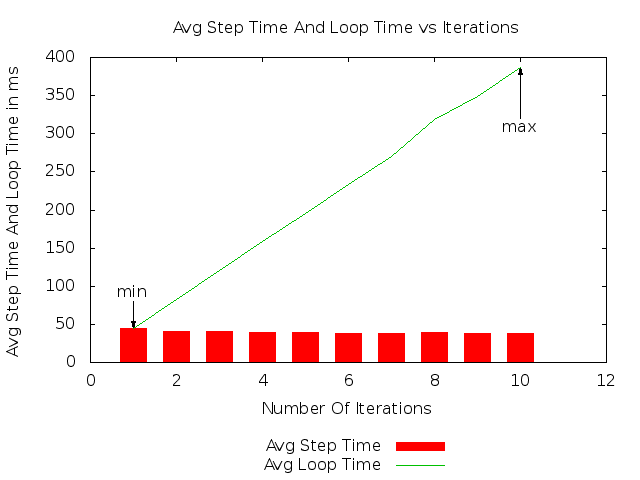
\includegraphics[height=7cm]{10_10_plot01.png}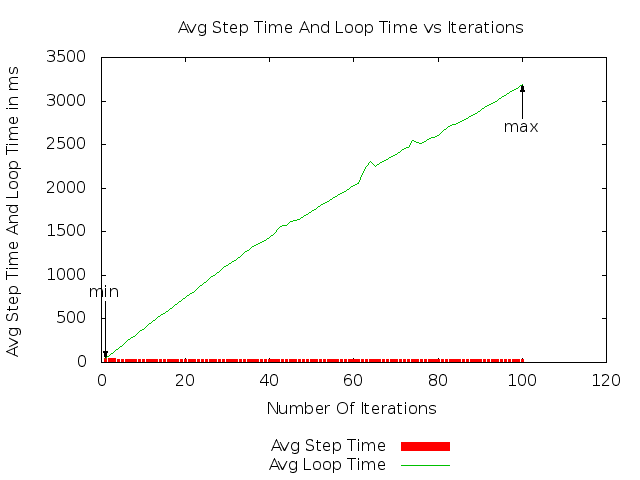
\includegraphics[height=7cm]{100_30_plot01.png}\end{center}

	\subsection{Analyzing Avg Time Taken To Resolve Velocity, Collision, Position Calculations And Avg Step Time}	
	The average time taken to resolve the velocity, collision and position values decreases with the increase in the number of iterations. This observation can be attributed to a reason similar to the reason for the decrease in avg step time with the increase in number of iterations. \newline
	\begin{equation*} AvgVelTime > AvgPosTime > AvgColTime \end{equation*} \newline
	Position vectors for objects can be found easily i.e. they are not calculation intensive. Velocity vectors for objects need to be continously calculated. For example the velocity vector for a sphere rolling on a surface with friction needs to be calculated continously (by continous we mean per small discrete amount of time). Determining the velocity vectors of two colliding objects is also a calculation intensive task. The Collision calculations will be done only when two objects collide (that is they only act as flags to determine whether two objects have collided or not). This explains the trend in the below graph.  
	
	\begin{center}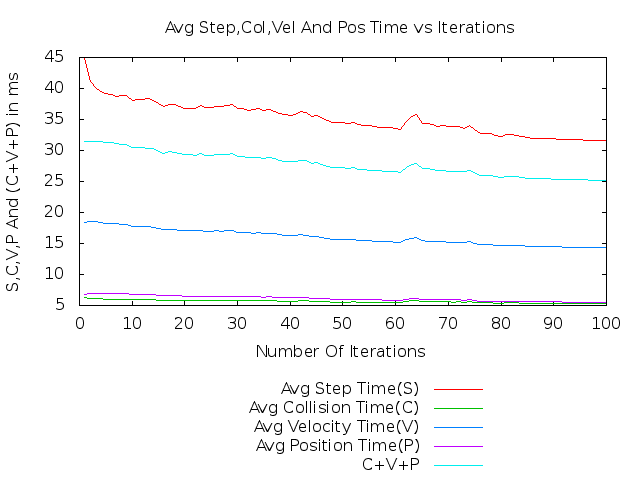
\includegraphics[height=8cm]{100_30_plot02.png}\end{center}

	\subsection{Analyzing Error Bars In Avg Step Time}
	From the below graph we observe that the relative error decreases as the iteration number increases. If we assume that the percentage error is constant i.e. it is independent of the iteration number, we can comment that the error decreases as the average step time itself decreases (Note: Here the rerun number is constant).
	As we increase the number of reruns the avg step time is closer to the actual step time. On the other hand the probability that we may get some noisy outputs increases. Hence if we compare two graphs with different rerun numbers (one with low and the other with high) the error in the graph with higher rerun number is expected to be greater (for a fixed iteration value). This can be particularly seen around iteration number 10-15. The graph on the left is for 30 reruns and the graph on the right is for 60 reruns. \newline

	\begin{center}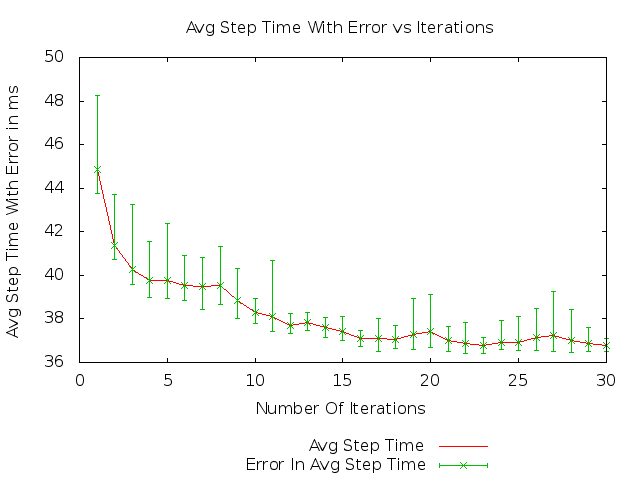
\includegraphics[height=7cm]{30_30_plot03.png}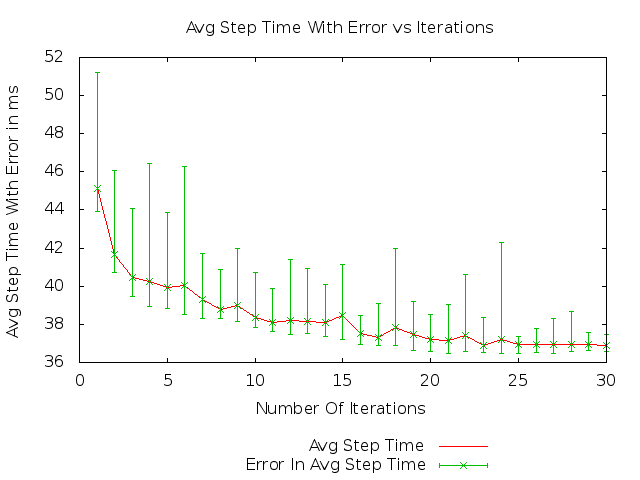
\includegraphics[height=7cm]{30_60_plot03.png}\end{center}
	
	\subsection{Analyzing The Frequency Plot For Avg Step Time}
	Most of the avg step times(for various rerun numbers) tend to lie in the same bucket as the actual avg step time. Whereas the points lying outside this bucket may have occured due to some noise in our measurements. Pure statistical analysis would suggest that the average step time for various rerun numbers should be a normal distribution.
	
	\begin{center}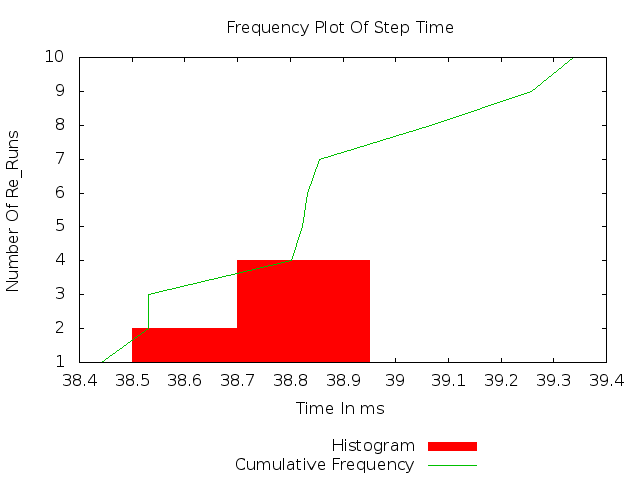
\includegraphics[height=7cm]{10_10_plot04.png}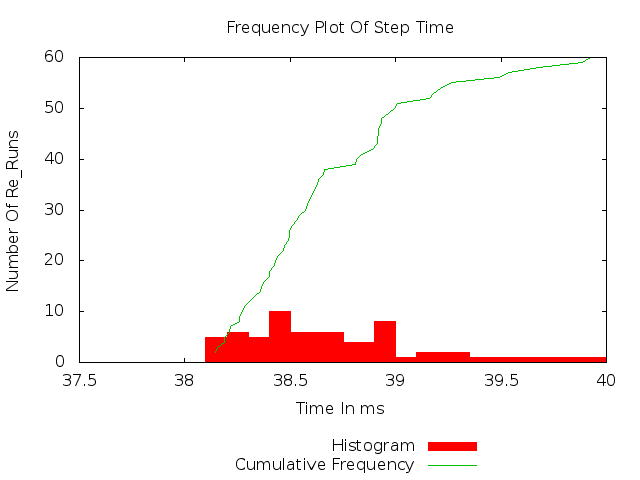
\includegraphics[height=7cm]{30_60_plot04.png}\end{center}

	\subsection{Analyzing Avg Step Time With A Random Sample}
	In the below graph we have plotted two things, one the average step time for all rerun values and the other the average step time over randomly selected reruns. There are two cases:-\newline
	Case1: When Number Of Iterations Is Large\newline
	In this case both the traces are almost similar due to which the best fit line is also almost the same for both. This mainly occurs because we have a lot of data points and the effect of a few outliers is nullified.\newline
	Case2: When Number Of Iterations Is Small\newline
	In this case we can see the difference in the graphs traced by the two type of data points. This difference is also reflected in the best fit lines.\newline
The above observations can be attributed to the fact that when we have lesser number of data points the tendency of getting an error is high whereas when we have a lot of data points the best fit lines for both the above cases tend to converge. The best fit lines also tend to converge as we increase the size of our random sample (for fixed number of iterations and reruns).
	
	\begin{center}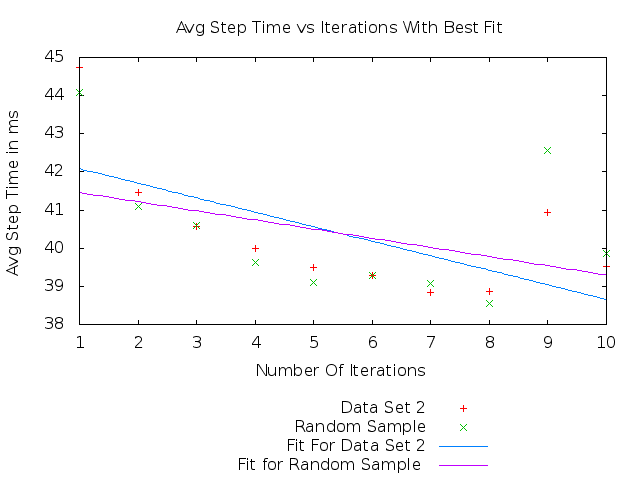
\includegraphics[height=7cm]{10_10_plot05.png}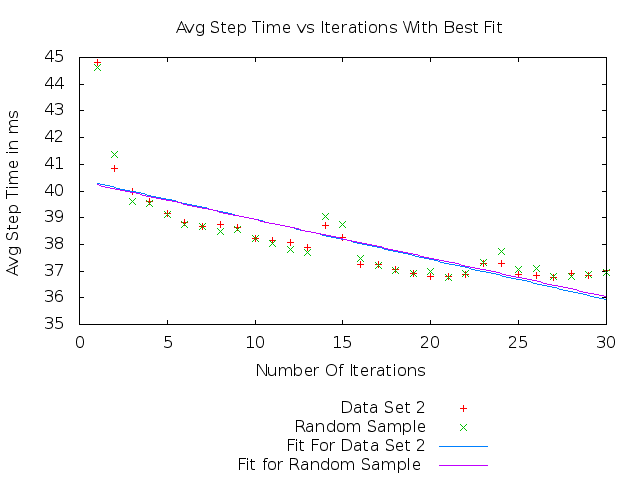
\includegraphics[height=7cm]{30_60_plot05.png}\end{center}

\section{Analyzing The Effect Of A Heavily Loaded System On Running Time}
	The time required to execute the base code without any parallel processes running on the system was much lesser than the time required to execute the base code with parallel processes running on the system. This suggested that the processes were executed in a thread like manner. By thread like manner we mean that if our process requires significant amount of time it is not executed in one shot but rather in parts.(Note: We loaded the system by running the base code for 1,000,000 iterations in another shell) 

\section{Analyzing Difference In Output Due To GetTimeOfDay And Time}
	Firstly the real time will \b{ALWAYS} be greater than the output we obtain from gettimeofday for our particular piece of code. This is because of the fact that gettimeofday gives us the time required for only running the for loop whereas the real time gives us the time for running the enitre code i.e. time for running other part of the code + time for running the for loop.\newline
	Secondly both the real time as well as gettimeofday include the time taken by the OS to run other processes in the middle of our process.\newline
	Thirdly there are two conflicting things, the user time + system time (both obtained from the time command) includes the time for running the entire process whereas it does not include the time taken by the OS to run other processes in the middle of our process. Whereas gettimeofday does not include the time required for running the entire code and includes the time taken by the OS to run other processes. This makes it difficult to compare between the two namely gettimeofday and user time + system time. In cases when the OS is not heavily loaded the user + system time is greater than the time obtained from gettimeofday and vice-versa.(Note: By gettimeofday we mean the time obtained by taking the difference of the two gettimeofday calls, one before and one after the for loop)
	
\section{Analyzing Our Simulation In The Debug Mode And The Release Mode}
	The -On flags i.e. -O2, -O3 flags are optimization flags. When we enable these flags the compiler tries to optimize the performance of the binary at the expense of compiltaion time and the ability to debug the program. Whereas when we do not enable these flags the compiler tries to reduce the cost of compilation.\newline
	In the Release mode we enable the optimization flags due to which the compilation takes relatively more time. When we run the base code for 1000 iterations the cumulative time taken is 4.19 sec (This may be different on different systems). Whereas in the Debug mode the compilation time is lesser and the compiler tries to optimize the binary file. When we run the base code for 1000 iterations the cumulative time taken is 30.28 sec which is much much more than its counterpart.\newline
	The function b2Vec2::b2Vec2(float, float) takes the maximum time in the Debug mode with a self time of 6.68 seconds which is not even called once in the Release mode!!! \newline
	In the Release mode about 60\% time is taken by function calls b2ContactSolver::SolveVelocityConstraints() and b2ContactSolver::SolvePositionConstraints() with a net time of 2.42 seconds whereas in the Debug mode the same function calls take a net time of 3.87 seconds. In the Debug mode b2ContactSolver::SolveVelocityConstraints() function calls a few operator functions whereas these operator functions are not called at all in the Release mode (further improving the execution time). This observation can be made with the help of the Call Graph generated in the profile Or with the help of Callee-Caller Graph about which we discuss in the next section. 
\begin{verbatim}
 Debug Profile
  %   cumulative   self              self     total           
 time   seconds   seconds    calls  ms/call  ms/call  name    
 22.08      6.68     6.68 645934982     0.00     0.00  b2Vec2::b2Vec2(float, float)
  9.81      9.65     2.97                              b2ContactSolver::SolveVelocityConstraints()
  7.20     11.84     2.18 204292053     0.00     0.00  operator-(b2Vec2 const&, b2Vec2 const&)
\end{verbatim} 


\begin{verbatim}
 Release Profile
  %   cumulative   self              self     total           
 time   seconds   seconds    calls  Ts/call  Ts/call  name    
 41.53      1.74     1.74                             b2ContactSolver::SolveVelocityConstraints()
 16.23      2.42     0.68                             b2ContactSolver::SolvePositionConstraints()
\end{verbatim}

\section{Analyzing The Callee-Caller Graph}
	In the Callee-Caller Graph the node contains information about the function name, percentage time spent in the function and all its children, the percentage of the running time spent in the function alone and the total number of times the function was called (including recursive calls). The edge contains information about the percentage of running time transfered from the child to the parent (if available) and the number of calls the parent function made to its child.\newline
	The major difference in the Calee-Caller graphs of the Debug mode and the Release mode is that in the Release mode the parent to child calls have been minimized (almost all have been removed). Moreover some function nodes which are present in the Debug mode are not present in the Release mode eg. operator$*$ and operator$+$ functions.\newline
	One Inference one can draw from the above observation is that when the compiler compiles the code in the Release mode it minimizes the nested function calls (by somehow providing the implementation of the child function to the parent function) i.e. the number of parent to child calls in the Debug mode is much greater than the parent to child calls in the Release mode. 

	\begin{figure}\begin{center}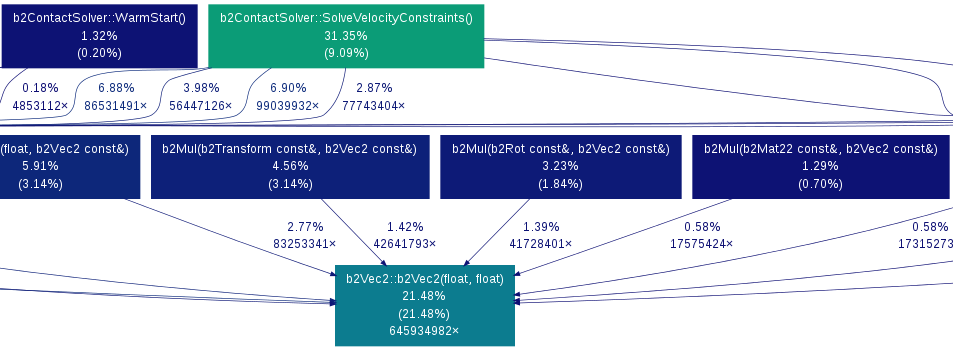
\includegraphics[height=5cm,width=20cm]{debug_1000_crop.png}\caption{Callee-Caller Graph For Debug Mode}\end{center}\end{figure}
	\begin{figure}\begin{center}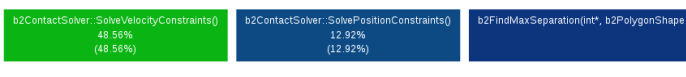
\includegraphics[height=1.5cm,width=15cm]{release_1000_crop.png}\caption{Callee-Caller Graph For Release Mode}\end{center}\end{figure}

\section{Things We Can Try To Optimize}
	We did an experiment, in the first case we removed the small boxes (representing dust) and profiled our code. In the second case we let the boxes be there and profiled our code. The cumulative time taken with the boxes was much more than the cumulative time taken without the boxes. This suggested that we should find an alternative to those small boxes. But to display the functionallity of our JCB the presence of those boxes is absouletly essential.\newline
	Moreover the function SolveVelocityConstraints takes the maximum time in the Release mode we should try to optimize this function for better running times.


\bibliographystyle{plain}
\bibliography{references}
\end{document}
		
